\chapter{Results}\label{chapter:results}
% Setup, supercomputers etc
% Profiler
% Memory usage maybe?
% Stream performance
% Mixed precision maybe?
% Hybrid solver?
% Different block sizes!!

This chapter presents results of the implementation of the adaptive \acrshort{acr:DG-SEM} wave
equation solver on \acrshort{acr:GPU} architectures and studies its effectiveness. Three main
components are studied. First, the performance of the core spectral element method code on
\acrshortpl{acr:GPU}, with a comparison with the same code running on \acrshortpl{acr:CPU} is
presented in Section~\ref{section:results:scaling_tests}. Then, the performance of the
\acrlong{acr:AMR} is studied in Section~\ref{section:results:adaptivity_performance}. Dynamic load
balancing is studied in Section~\ref{section:results:load_balancing_performance}. Finally, a more
complex application is shown in Section~\ref{section:results:complex_application}

\section{Platforms}\label{section:results:platforms}

The implementation we have developed aims to perform large scale computations, and as such targets
\acrshort{acr:HPC} platforms. The program has been designed to scale to multiple levels of
parallelism, the highest being splitting the workload between several \acrshort{acr:HPC} nodes, each
having multiple \acrshortpl{acr:CPU} and \acrshortpl{acr:GPU}. To test this use case, most of the
following tests were run on clusters graciously offered by Compute
Canada\footnote{https://www.computecanada.ca/}. Two such clusters were used for our experiments,
Béluga and Narval.

\subsection{Béluga}\label{subsection:results:platforms:beluga}

Béluga is a heterogeneous cluster suitable for a variety of purposes, from traditional
\acrshort{acr:CPU} computing to massively parallel \acrshort{acr:GPU} computing. It is located at
the École de technologie supérieure in Montréal. Béluga is made up of 977 compute nodes of different
types, totaling 39,120 \acrshort{acr:CPU} cores and 696 \acrshortpl{acr:GPU}. For our testing, we
use Béluga's general usage \acrshort{acr:GPU} nodes. Each one of the 172 \acrshort{acr:GPU} nodes
contains 40 \acrshort{acr:CPU} cores and 186 GB of memory across two Intel Gold 6148
\acrshortpl{acr:CPU}, and four NVidia V100 SXM2 \acrshortpl{acr:GPU} with 16 GB of memory each. One
such node totals about 2 TFlops of double precision \acrshort{acr:CPU} computing power, and 13
TFlops of double precision \acrshort{acr:GPU} computing power. The nodes are connected by Infiniband
HDR (100 Gb/s) interconnections.

\subsection{Narval}\label{subsection:results:platforms:narval}

Narval is a heterogeneous cluster suitable for a variety of purposes, from traditional
\acrshort{acr:CPU} computing to massively parallel \acrshort{acr:GPU} computing and artificial
intelligence workloads. It is located at the École de technologie supérieure in Montréal. Narval is
made up of 1301 compute nodes of different types, totaling 80,720 \acrshort{acr:CPU} cores and 636
\acrshortpl{acr:GPU}. For our testing, we use Narval's \acrshort{acr:GPU} nodes. Each one of the 159
\acrshort{acr:GPU} nodes contains 48 \acrshort{acr:CPU} cores and 498 GB of memory across two AMD
Milan 7413 \acrshortpl{acr:CPU}, and four NVidia A100 \acrshortpl{acr:GPU} with 40 GB of memory
each. One such node totals about 2.2 TFlops of double precision \acrshort{acr:CPU} computing power,
and 38.8 TFlops of double precision \acrshort{acr:GPU} computing power. The nodes are connected by
Infiniband EDR (100 Gb/s) interconnections.

\subsection{Consumer hardware}\label{subsection:results:platforms:consumer}

Some smaller scale tests or tests that did not involve performance were run on consumer hardware.
This is important, as it may not always be possible to access \acrshort{acr:HPC} systems when flow
simulations have to be performed. The program should also have reasonable performance on regular
systems. The system used in these cases is a single computer containing 16 \acrshort{acr:CPU} cores
and 128 GB of memory across two Intel E5\textendash2650 V2 \acrshortpl{acr:CPU}, and one NVidia GTX
1070 \acrshort{acr:GPU} with 8 GB of memory. This totals about 0.5 TFlops of double precision
\acrshort{acr:CPU} computing power, and 0.25 TFlops of double precision \acrshort{acr:GPU} computing
power. This is an interesting comparison, as consumer \acrshortpl{acr:GPU} are not geared towards
high precision compute loads. \Acrshortpl{acr:GPU} found in \acrshort{acr:HPC} systems typically
have a 1:2 ratio between their double precision and single precision performance, whereas consumer
\acrshortpl{acr:GPU} usually have 1:32 ratio. This means that computations using double precision
floating point numbers will execute at one sixteenth of the speed of compute-oriented
\acrshortpl{acr:GPU}, all other factors being equal.

\section{Test case}\label{section:results:test_case}
% new case

\begin{figure}[H]
	\centering
	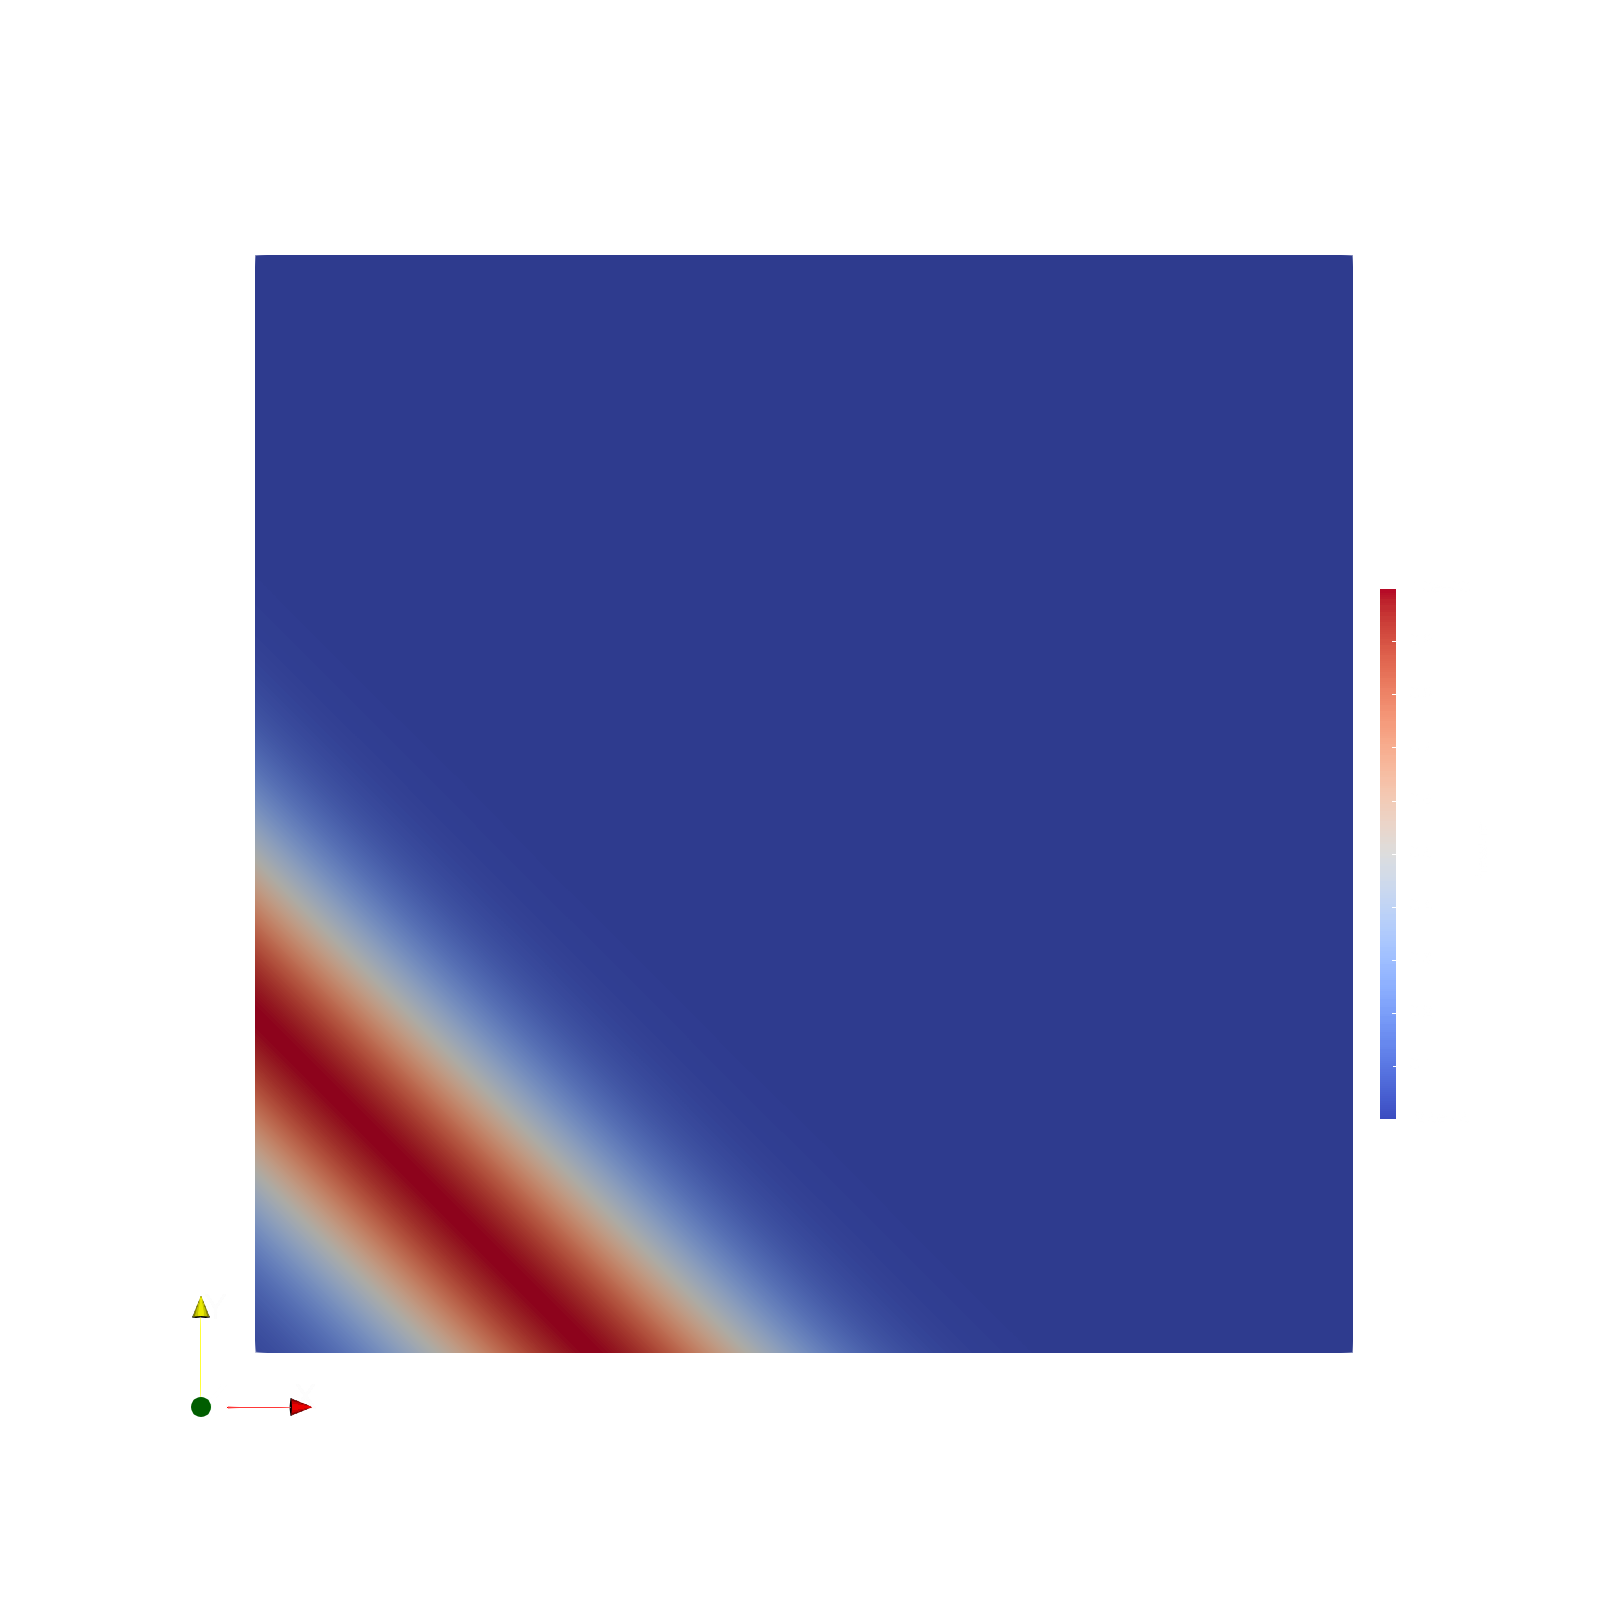
\includegraphics[width=0.6\textwidth]{Chapter_results/media/problem_1}
	\caption{Test case: A wave travels through a square domain at a 45° angle.}\label{fig:problem}
\end{figure}

\section{Scaling tests}\label{section:results:scaling_tests}
% Scaling tests (strong and weak), N tests
% CPU vs GPU
% GPU loading

Parallel scaling is an important aspect of the performance of a program. It describes how the
execution time varies when more resources are assigned to the problem. This is an optimisation
problem, as each problem will have an optimal amount of resources dedicated to it. 

A completely parallelisable program, often called embarrassingly parallel, should scale linearly
with the amount of resources. The speedup \(S\) of a workload split between \(W\) workers should be
equal to the number of workers in Equation~\ref{equ:scaling}. In this work, workers are a single
\acrshort{acr:GPU} or a single \acrshort{acr:CPU} core for comparative tests.

\begin{equation} \label{equ:scaling}
	S = \frac{t_1}{t_W}
\end{equation}

Unfortunately, it is often not possible to make a program entirely parallel. In such cases, dividing
a problem into more and more smaller tasks obeys the well-known Amdahl's law~\cite{Amdahl1967}, as
seen in Equation~\ref{equ:strong_scaling}. It splits the program into a sequential part \(s\) and a
parallel part \(p\), with only the parallel part scaling with the number of workers.

\begin{equation} \label{equ:strong_scaling}
	S = \frac{1}{s + \frac{p}{W}}
\end{equation}

This is called \textit{strong scaling}, where a fixed problem is solved using varying amount of
resources. This is discussed in Subsection~\ref{subsection:results:scaling_tests:strong}.

On the other hand, increased available resources can enable working on bigger problems. Gustafson
argues that modern highly parallel computers will be used to solve more complex problems instead of
solving smaller problems faster. Such a scaling is described with Equation~\ref{equ:weak_scaling}.

\begin{equation} \label{equ:weak_scaling}
	S = s + p \times W
\end{equation}

This is called \textit{weak scaling}. It describes solving a problem whose size increases with the
amount of resources, with the task size per worker stays constant. Weak scaling is tested in
Subsection~\ref{subsection:results:scaling_tests:weak}. With weak scaling a program will scale
indefinitely, with the slope of the scaling being influenced by the parallel proportion of the task.

This section will also serve as a general comparison between \acrshortpl{acr:CPU} and
\acrshortpl{acr:GPU}. All scaling tests have been performed on the Béluga supercomputer. Scaling is
evaluated by varying the number of \textit{nodes}, where a node in this context is a single computer
from Béluga, sporting 40 \acrshort{acr:CPU} cores and 4 \acrshortpl{acr:GPU}, as stated in
Subsection~\ref{subsection:results:platforms:beluga}. The four-node execution time of those tests
therefore represents the program running on 16 \acrshortpl{acr:GPU} or 160 \acrshort{acr:CPU} cores,
for the \acrshort{acr:GPU} and \acrshort{acr:CPU} computations respectively.

Both scaling tests evaluate the core solver part of the program, as the meshes start with enough
elements to have a well resolved solution all along the simulation. The \acrlong{acr:AMR} and
dynamic load balancing subroutines are still enabled. The subroutines still run their evaluation
phases, the error estimation and load imbalance computation respectively, but do not deem the
estimated error and load imbalance high enough to trigger the whole subroutine. 

\subsection{Strong scaling}\label{subsection:results:scaling_tests:strong}

The test case for this section is described in Section~\ref{section:results:test_case}. It is
divided into 256 elements in the \(x\) and \(y\) direction, for a total of \(K = 65536\). The
problem is then solved in parallel from one quarter node to eight nodes. One quarter node contains 1
\acrshort{acr:GPU} and 10 \acrshort{acr:CPU} cores, while eight nodes contain 16
\acrshortpl{acr:GPU} and 160 \acrshort{acr:CPU} cores. The mesh is split into blocks accordingly,
one block per \acrshort{acr:GPU} or one block per \acrshort{acr:CPU} core. The first test has a
polynomial order \(N\) of four for all elements, and a block size \(B\) of 32. 

The block size, as explained in
Subsection~\ref{subsection:graphics_processing_units:architecture:programming_model}, is the number
of threads in a block of threads. Having a higher block size can speed up execution by reducing the
number of instructions to dispatch by the control flow unit of the \acrshort{acr:GPU}, because the
instructions are dispatched by block of threads. However, if the threads within a block diverge,
having a higher block size can actually lower performance. A single thread diverging will have all
the threads in its block waiting until it is finished, therefore a higher block size will have more
threads stalled when divergence occurs.

All tests have an ``ideal'' line both for the \acrshort{acr:GPU} and \acrshort{acr:CPU}
calculations. This line represents the optimal split for that case, with the number of nodes with
the best scaling, extrapolated linearly to the other splits.

\begin{figure}[H]
	\centering
	\includesvg[width=0.6\textwidth]{Chapter_results/media/strong_scaling_N4_K65536_W32}
	\caption{Weak scaling: The problem size increases with the number of workers. N = 4, K = 65536, B = 32}\label{fig:strong_scaling_N4_W32}
\end{figure}

Figure~\ref{fig:strong_scaling_N4_W32} shows that the \acrshort{acr:GPU} implementation, initially
slower than the \acrshort{acr:CPU} implementation, overtakes it when one full node or more is used.
The higher number of nodes show the \acrshort{acr:GPU} implementation to be \(2.9 \times \) faster
that the \acrshort{acr:CPU} implementation.

At low numbers of \acrshortpl{acr:GPU} working on the same problem, the \acrshortpl{acr:GPU} are
more heavily loaded. It is possible that the higher memory usage, or the increased cache eviction
rate lowers the performance of \acrshortpl{acr:GPU} in that regime. With a lower number of elements
being worked on by a \acrshort{acr:GPU}, cache has to be emptied less often to make room for more
elements to use for computations.

At the end of the curve, we see that the scaling lowers slightly. This could be a hint that the
\acrshortpl{acr:GPU} are then not loaded enough. These \acrshortpl{acr:GPU} have many
\acrshort{acr:CUDA} cores, 5120 each in the case of Béluga. If the workload does not saturate
the \acrshort{acr:GPU}, some of those cores will be idle, leading to worse performance. The optimal
number of elements per \acrshort{acr:GPU} seems to be around 4096.

The next test, shown on Figure~\ref{fig:strong_scaling_N6_W32}, shows the same test case but with an
increased polynomial order of \(N = 6\) for all elements. The rationale is that the
\acrshort{acr:GPU} should spend more time on the computations, since the computations will be
heavier, while spending the same time on the overhead of kernel calls and other housekeeping.

\begin{figure}[H]
	\centering
	\includesvg[width=0.6\textwidth]{Chapter_results/media/strong_scaling_N6_K65536_W32}
	\caption{Weak scaling: The problem size increases with the number of workers. N = 6, K = 65536, B = 32}\label{fig:strong_scaling_N6_W32}
\end{figure}

Figure~\ref{fig:strong_scaling_N6_W32} shows that the increased polynomial order has not increased
the performance of the \acrshort{acr:GPU} implementation compared to the \acrshort{acr:CPU}
implementation, rather shifting to the right the crossover point where the \acrshort{acr:GPU}
implementation is faster. It is possible that the reduced relative performance is linked to the
increased memory used by the solution, as the needed storage is relative to \(2 N + 1\), where \(N\)
is the polynomial order of elements.

Next, this last case is computer again with increased block size \(B\), first 64 on
Figure~\ref{fig:strong_scaling_N6_W64}, then 128 on Figure~\ref{fig:strong_scaling_N6_W128}. The
\acrshort{acr:CPU} implementation is not modified. This should assess the incidence of block size on
the solution time.

\begin{figure}[H]
	\centering
	\includesvg[width=0.6\textwidth]{Chapter_results/media/strong_scaling_N6_K65536_W64}
	\caption{Weak scaling: The problem size increases with the number of workers. N = 6, K = 65536, B = 64}\label{fig:strong_scaling_N6_W64}
\end{figure}

\begin{figure}[H]
	\centering
	\includesvg[width=0.6\textwidth]{Chapter_results/media/strong_scaling_N6_K65536_W128}
	\caption{Weak scaling: The problem size increases with the number of workers. N = 6, K = 65536, B = 128}\label{fig:strong_scaling_N6_W128}
\end{figure}

A the last two figures suggest, increasing the block size \(B\) does incur a performance penalty.
This is possible caused by a high amount of thread divergence within blocks. This is consistent with
how the program is written, for example
Section~\ref{section:adaptive_mesh_refinement:implementation} shows how the projection back and
forth between the elements and faces have a low of branching code paths. A lot of changes in the
architecture of the program would have to be made to reduce this branching, and switch to a more
data-driven approach.

One thing to note is that the curve of the \acrshort{acr:CPU} implementation on
Figures~\ref{fig:strong_scaling_N4_W32} and~\ref{fig:strong_scaling_N6_W32} is similar, whereas the
\acrshort{acr:GPU} curves from all the figures differ significantly. This is a recurring theme of
all the tests in this chapter, code running on \acrshortpl{acr:GPU} seems to be harder to optimise
and some factors have unexpected influences on the performance.

\subsection{Weak scaling}\label{subsection:results:scaling_tests:weak}

The weak scaling test uses the text case from Section~\ref{section:results:test_case}. The domain is
split up into elements such that each node contains 16384 elements. This amounts to 4096 elements
per \acrshort{acr:GPU}, or 410 elements per \acrshort{acr:CPU} core. The simulation is first
computed with the highest number of nodes, therefore the smallest elements and time step size. The
\acrshort{acr:CFL} number is adjusted for all other simulations to get the same time step size,
therefore the same total number of iterations. An ideal result is a flat curve, indicating that by
increasing the problem size and resources by the same amount, the simulation time stays the same.
The problem is studied from ¼ node to 16 nodes.

\begin{figure}[H]
	\centering
	\includesvg[width=0.6\textwidth]{Chapter_results/media/weak_scaling_N4_K4096_W32}
	\caption{Weak scaling: The problem size increases with the number of workers. N = 4, K = 16384/node}\label{fig:weak_scaling}
\end{figure}

Figure~\ref{fig:weak_scaling} shows good weak scaling from the \acrshort{acr:GPU} implementation.
Keeping in mind that the quarter node and single node cases have a reduced workload by not having to
do any \acrshort{acr:MPI} communication over the network, and the quarter node \acrshort{acr:GPU}
case has no \acrshort{acr:MPI} communication to do at all, the \acrshort{acr:GPU} curve is
reasonably flat. The \acrshort{acr:CPU} curve is not as good, indicating that there may be a
bottleneck in the communication part of the program. The \acrshort{acr:CPU} implementation has a
much higher number of workers than the \acrshort{acr:GPU} one, 40 per node instead of four,
increasing the inter-process communication needed. The slope of the \acrshort{acr:CPU} curve is
about \(0.2\) with regards to the number of \acrshort{acr:CPU} cores. 

\section{Adaptive mesh refinement performance}\label{section:results:adaptivity_performance}
% Error adaptive vs non-adaptive, time to run
% Error at same runtime

This section establishes the performance of the \acrlong{acr:AMR}. The problem from
Section~\ref{section:results:test_case} is used, initially split into four elements in the \(x\) and
\(y\) direction, for \(K = 16\). The initial polynomial order \(N\) of four. The system is allowed
to refine up to a split level of three, meaning a cell can split three times and become one eighth
the size of the original cell, and up to a polynomial order \(N\) of 12.

\Acrlong{acr:AMR} is a costly process, as the \acrshort{acr:CPU} must reallocate arrays on the
\acrshort{acr:GPU} for the different objects making up the mesh, and then schedule kernels to move
objects to the new arrays. We test here two strategies to reduce the performance overhead of
\acrlong{acr:AMR}, while reducing error. 

First, \acrlong{acr:AMR} will be performed at an interval.
Figures~\ref{fig:adaptivity_efficiency_C5},~\ref{fig:adaptivity_efficiency_C20},~\ref{fig:adaptivity_efficiency_C100}
and~\ref{fig:adaptivity_efficiency_C500} show the results of refining the mesh every 5, 20, 100 and
500 timesteps, respectively.

Secondly, the simulations are performed with an increasing number of refinement pre-conditioning
steps as described in Section~\ref{section:adaptive_mesh_refinement:pre_conditioning}. The analysis
ranges from no pre-conditioning step to three steps.

We compare those simulation to a non-adaptive case, where the initial mesh is refined uniformly to
the maximum level attained by the adaptive case. The mesh is split into 32 elements in the \(x\) and
\(y\) dimensions, for  \(K = 1024\), with a polynomial order  \(N\) of 10. Both the simulation time
and the error against the analytical solution are compared. The non-adaptive case is shown as a
dotted line on the figures.

\begin{figure}[H]
	\centering
	\includesvg[width=0.6\textwidth]{Chapter_results/media/adaptivity_N4_K16_C5}
	\caption{Adaptivity efficiency: Simulation time and analytical error with adaptivity and increasing pre-processing steps. N = 4, K = 16, adaptivity interval = 5}\label{fig:adaptivity_efficiency_C5}
\end{figure}

\begin{figure}[H]
	\centering
	\includesvg[width=0.6\textwidth]{Chapter_results/media/adaptivity_N4_K16_C20}
	\caption{Adaptivity efficiency: Simulation time and analytical error with adaptivity and increasing pre-processing steps. N = 4, K = 16, adaptivity interval = 20}\label{fig:adaptivity_efficiency_C20}
\end{figure}

\begin{figure}[H]
	\centering
	\includesvg[width=0.6\textwidth]{Chapter_results/media/adaptivity_N4_K16_C100}
	\caption{Adaptivity efficiency: Simulation time and analytical error with adaptivity and increasing pre-processing steps. N = 4, K = 16, adaptivity interval = 100}\label{fig:adaptivity_efficiency_C100}
\end{figure}

\begin{figure}[H]
	\centering
	\includesvg[width=0.6\textwidth]{Chapter_results/media/adaptivity_N4_K16_C500}
	\caption{Adaptivity efficiency: Simulation time and analytical error with adaptivity and increasing pre-processing steps. N = 4, K = 16, adaptivity interval = 500}\label{fig:adaptivity_efficiency_C500}
\end{figure}

From
Figures~\ref{fig:adaptivity_efficiency_C5},~\ref{fig:adaptivity_efficiency_C20},~\ref{fig:adaptivity_efficiency_C100}
and~\ref{fig:adaptivity_efficiency_C500}, we can that this is an optimisation problem, with
tradeoffs between the simulation time and the error generated.

In all cases, without pre-conditioning, increasing the adaptivity interval reduces the simulation
time, but increases error. Even with 

\section{Dynamic load balancing performance}\label{section:results:load_balancing_performance}
% Runtime adaptive with and without load balancing

Max split level  \(S\). Where  \(K_p\) is the number of elements in process  \(p\).

\begin{figure}[H]
	\centering
	\subfloat[Pressure]
	{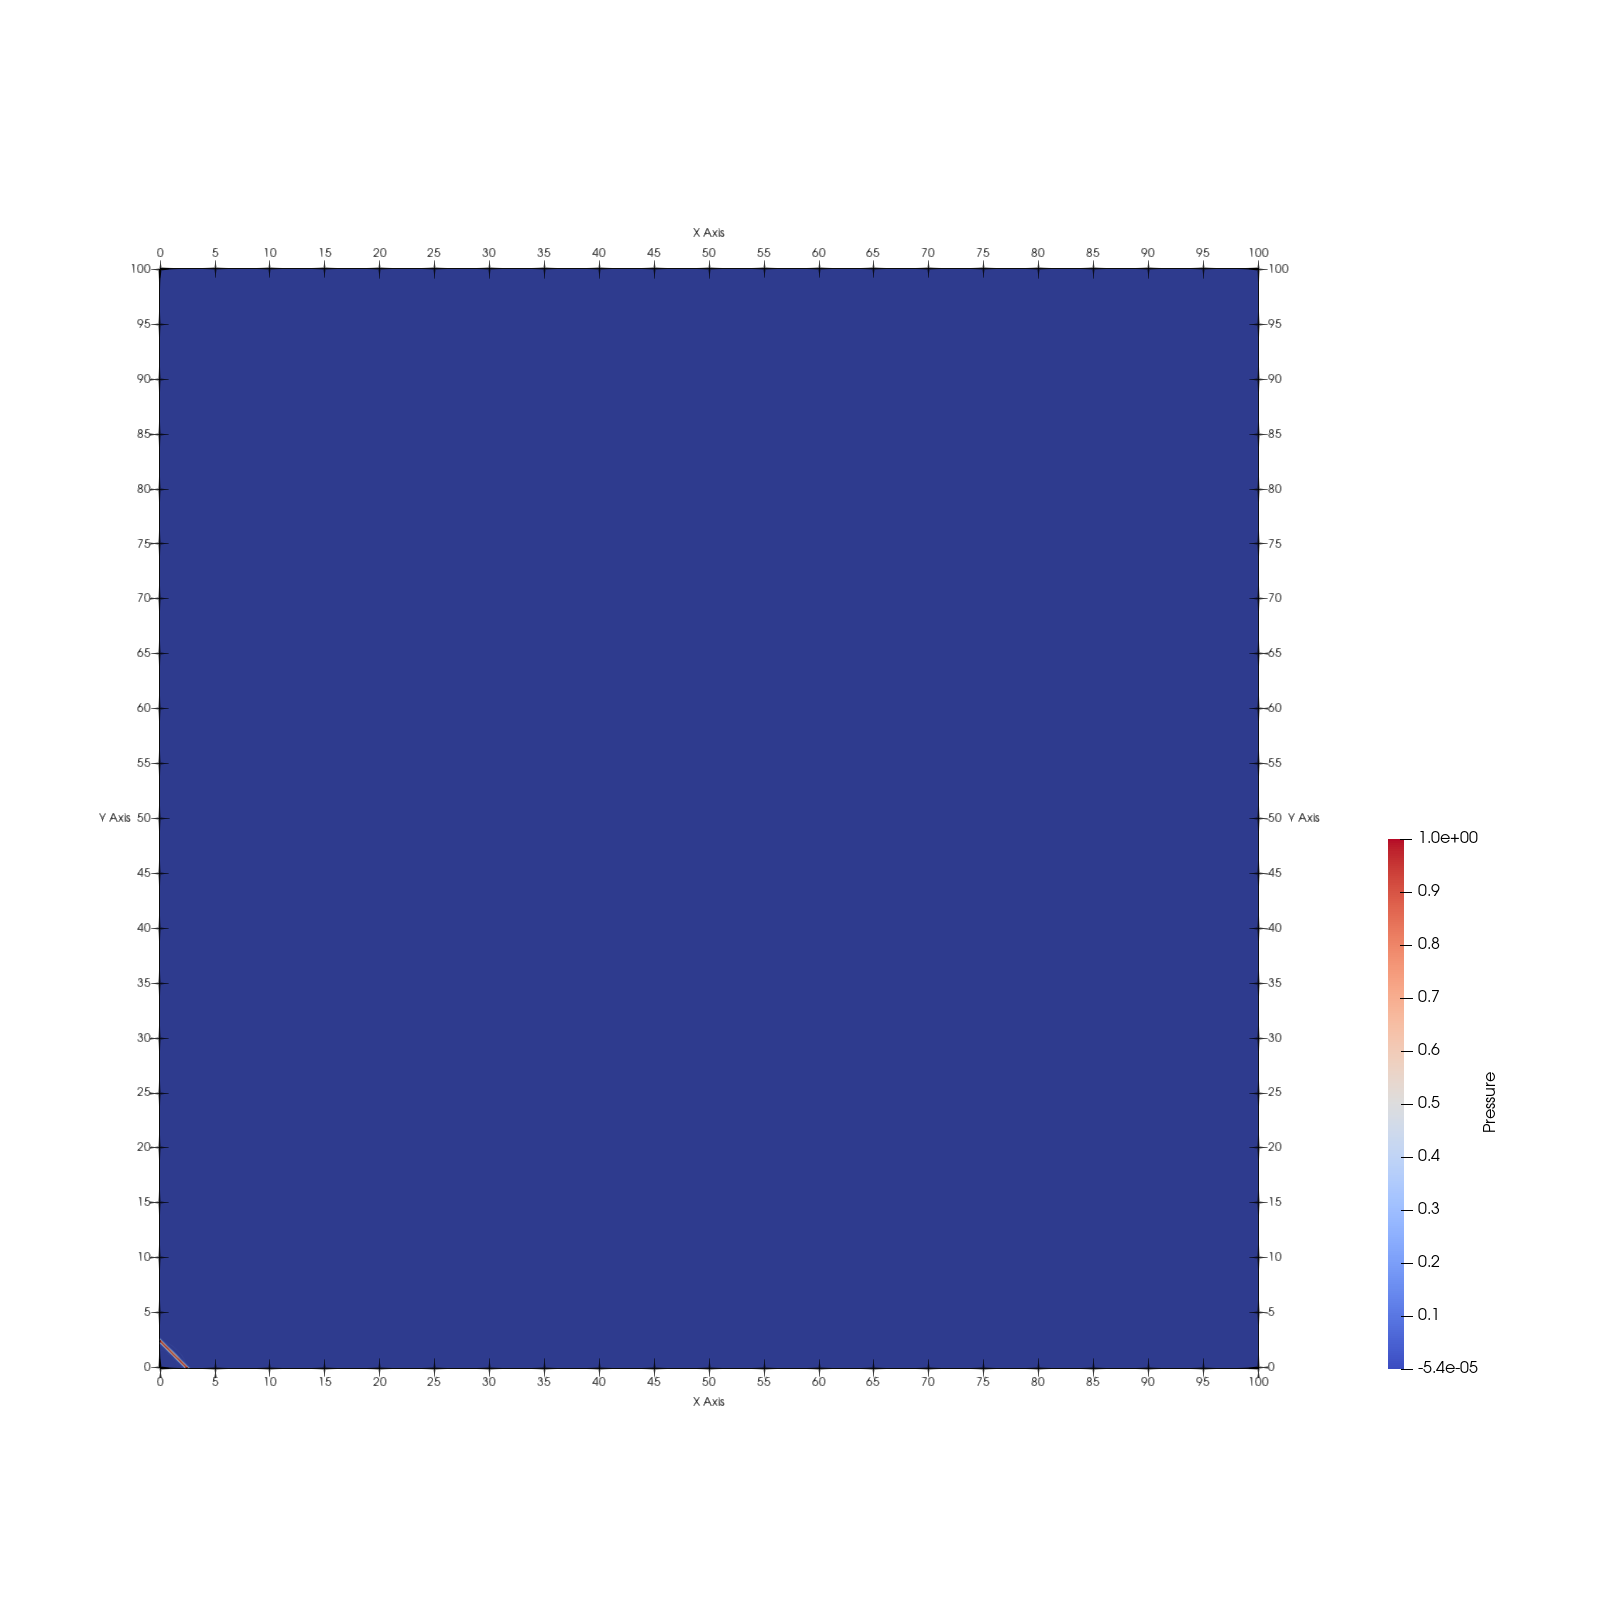
\includegraphics[width=0.45\textwidth]{Chapter_results/media/problem_big}\label{fig:load_imbalance_case_p}}
	\hfill
	\subfloat[Split level]
	{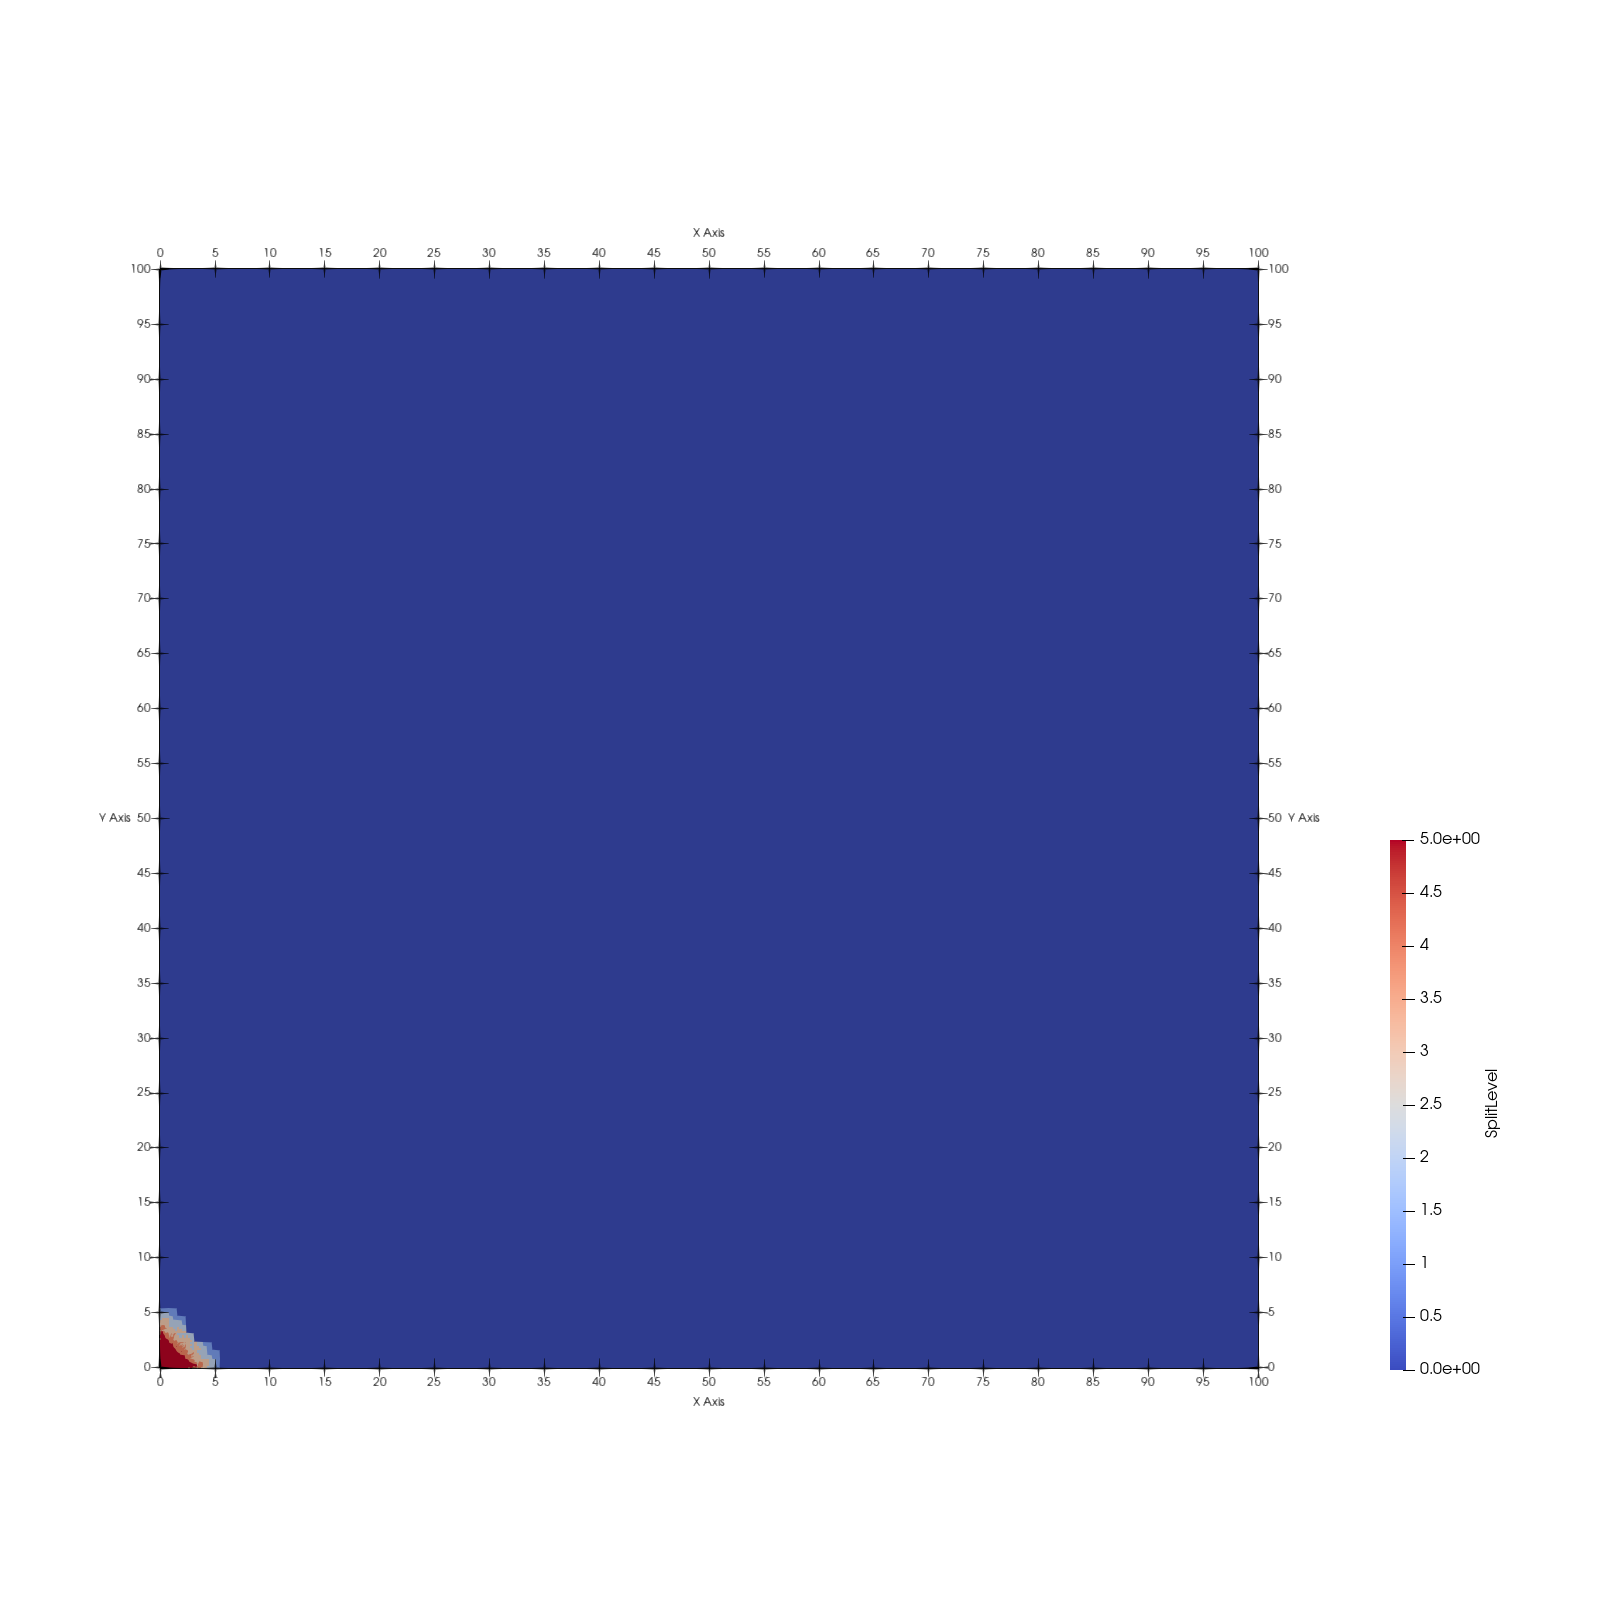
\includegraphics[width=0.45\textwidth]{Chapter_results/media/split_level_big}\label{fig:load_imbalance_case_s}}
	\caption{Load imbalance test case: A wave passes through a very big domain, only the bottom right refines. (a) Pressure (b) Split level, indicating how many times the elements have split}\label{fig:load_imbalance_case}
\end{figure}

\begin{table}[H]
	\centering
	\begin{tabular}{ c c c c c c c }
		Case & S & K & Max \(K_p\) & Min \(K_p\) & Load imbalance & Imbalance ratio \\
		\midrule
		Low & \(3\) & \(17752\) & \(2392\) & \(1024\) & \(2.34\) & \(2.16\) \\
		High & \(5\) & \(26734\) & \(11374\) & \(1024\) & \(11.1\) & \(6.81\) \\
	\end{tabular}
	\caption{Load imbalance cases.}\label{table:load_imbalance}
\end{table}

\subsection{Load balancing interval}\label{subsection:results:load_balancing_performance:interval}

\begin{figure}[H]
	\centering
	\includesvg[width=0.6\textwidth]{Chapter_results/media/load_balancing_interval_N4_K16384_A20_P16_S3}
	\caption{Load balancing efficiency interval test: Simulation time with adaptivity, load balancing and increasing load balancing interval. N = 4, K = 16384, adaptivity interval = 20, W = 16, max split level = 3}\label{fig:load_balancing_efficiency_interval}
\end{figure}

\begin{figure}[H]
	\centering
	\includesvg[width=0.6\textwidth]{Chapter_results/media/load_balancing_interval_N4_K16384_A20_P16_S5}
	\caption{Load balancing efficiency interval test: Simulation time with adaptivity, load balancing and increasing load balancing interval. N = 4, K = 16384, adaptivity interval = 20, W = 16, max split level = 3}\label{fig:load_balancing_efficiency_interval_s5}
\end{figure}

% Say that the interval depends on the problem size

\subsection{Load balancing threshold}\label{subsection:results:load_balancing_performance:threshold}

\begin{figure}[H]
	\centering
	\includesvg[width=0.6\textwidth]{Chapter_results/media/load_balancing_threshold_N4_K16384_A20_L20_P16_S3}
	\caption{Load balancing efficiency threshold test: Simulation time with adaptivity, load balancing and increasing load balancing threshold. N = 4, K = 16384, adaptivity interval = 20, load balancing interval = 20, W = 16, max split level = 3}\label{fig:load_balancing_efficiency_threshold_s3}
\end{figure}

\begin{figure}[H]
	\centering
	\includesvg[width=0.6\textwidth]{Chapter_results/media/load_balancing_threshold_N4_K16384_A20_L20_P16_S5}
	\caption{Load balancing efficiency threshold test: Simulation time with adaptivity, load balancing and increasing load balancing threshold. N = 4, K = 16384, adaptivity interval = 20, load balancing interval = 20, W = 16, max split level = 3}\label{fig:load_balancing_efficiency_threshold_s5}
\end{figure}

\subsection{Polynomial order influence}\label{subsection:results:load_balancing_performance:polynomial_order}

\begin{figure}[H]
	\centering
	\includesvg[width=0.6\textwidth]{Chapter_results/media/N_iteration_time}
	\caption{Polynomial order influence: Iteration time with increasing polynomial order.}\label{fig:N_influence}
\end{figure}

\section{Complex application}\label{section:results:complex_application}

\section{Complex meshes}\label{section:results:complex_meshes}
% Move to annex

\begin{figure}[H]
	\centering
	\subfloat[Circular domain]
	{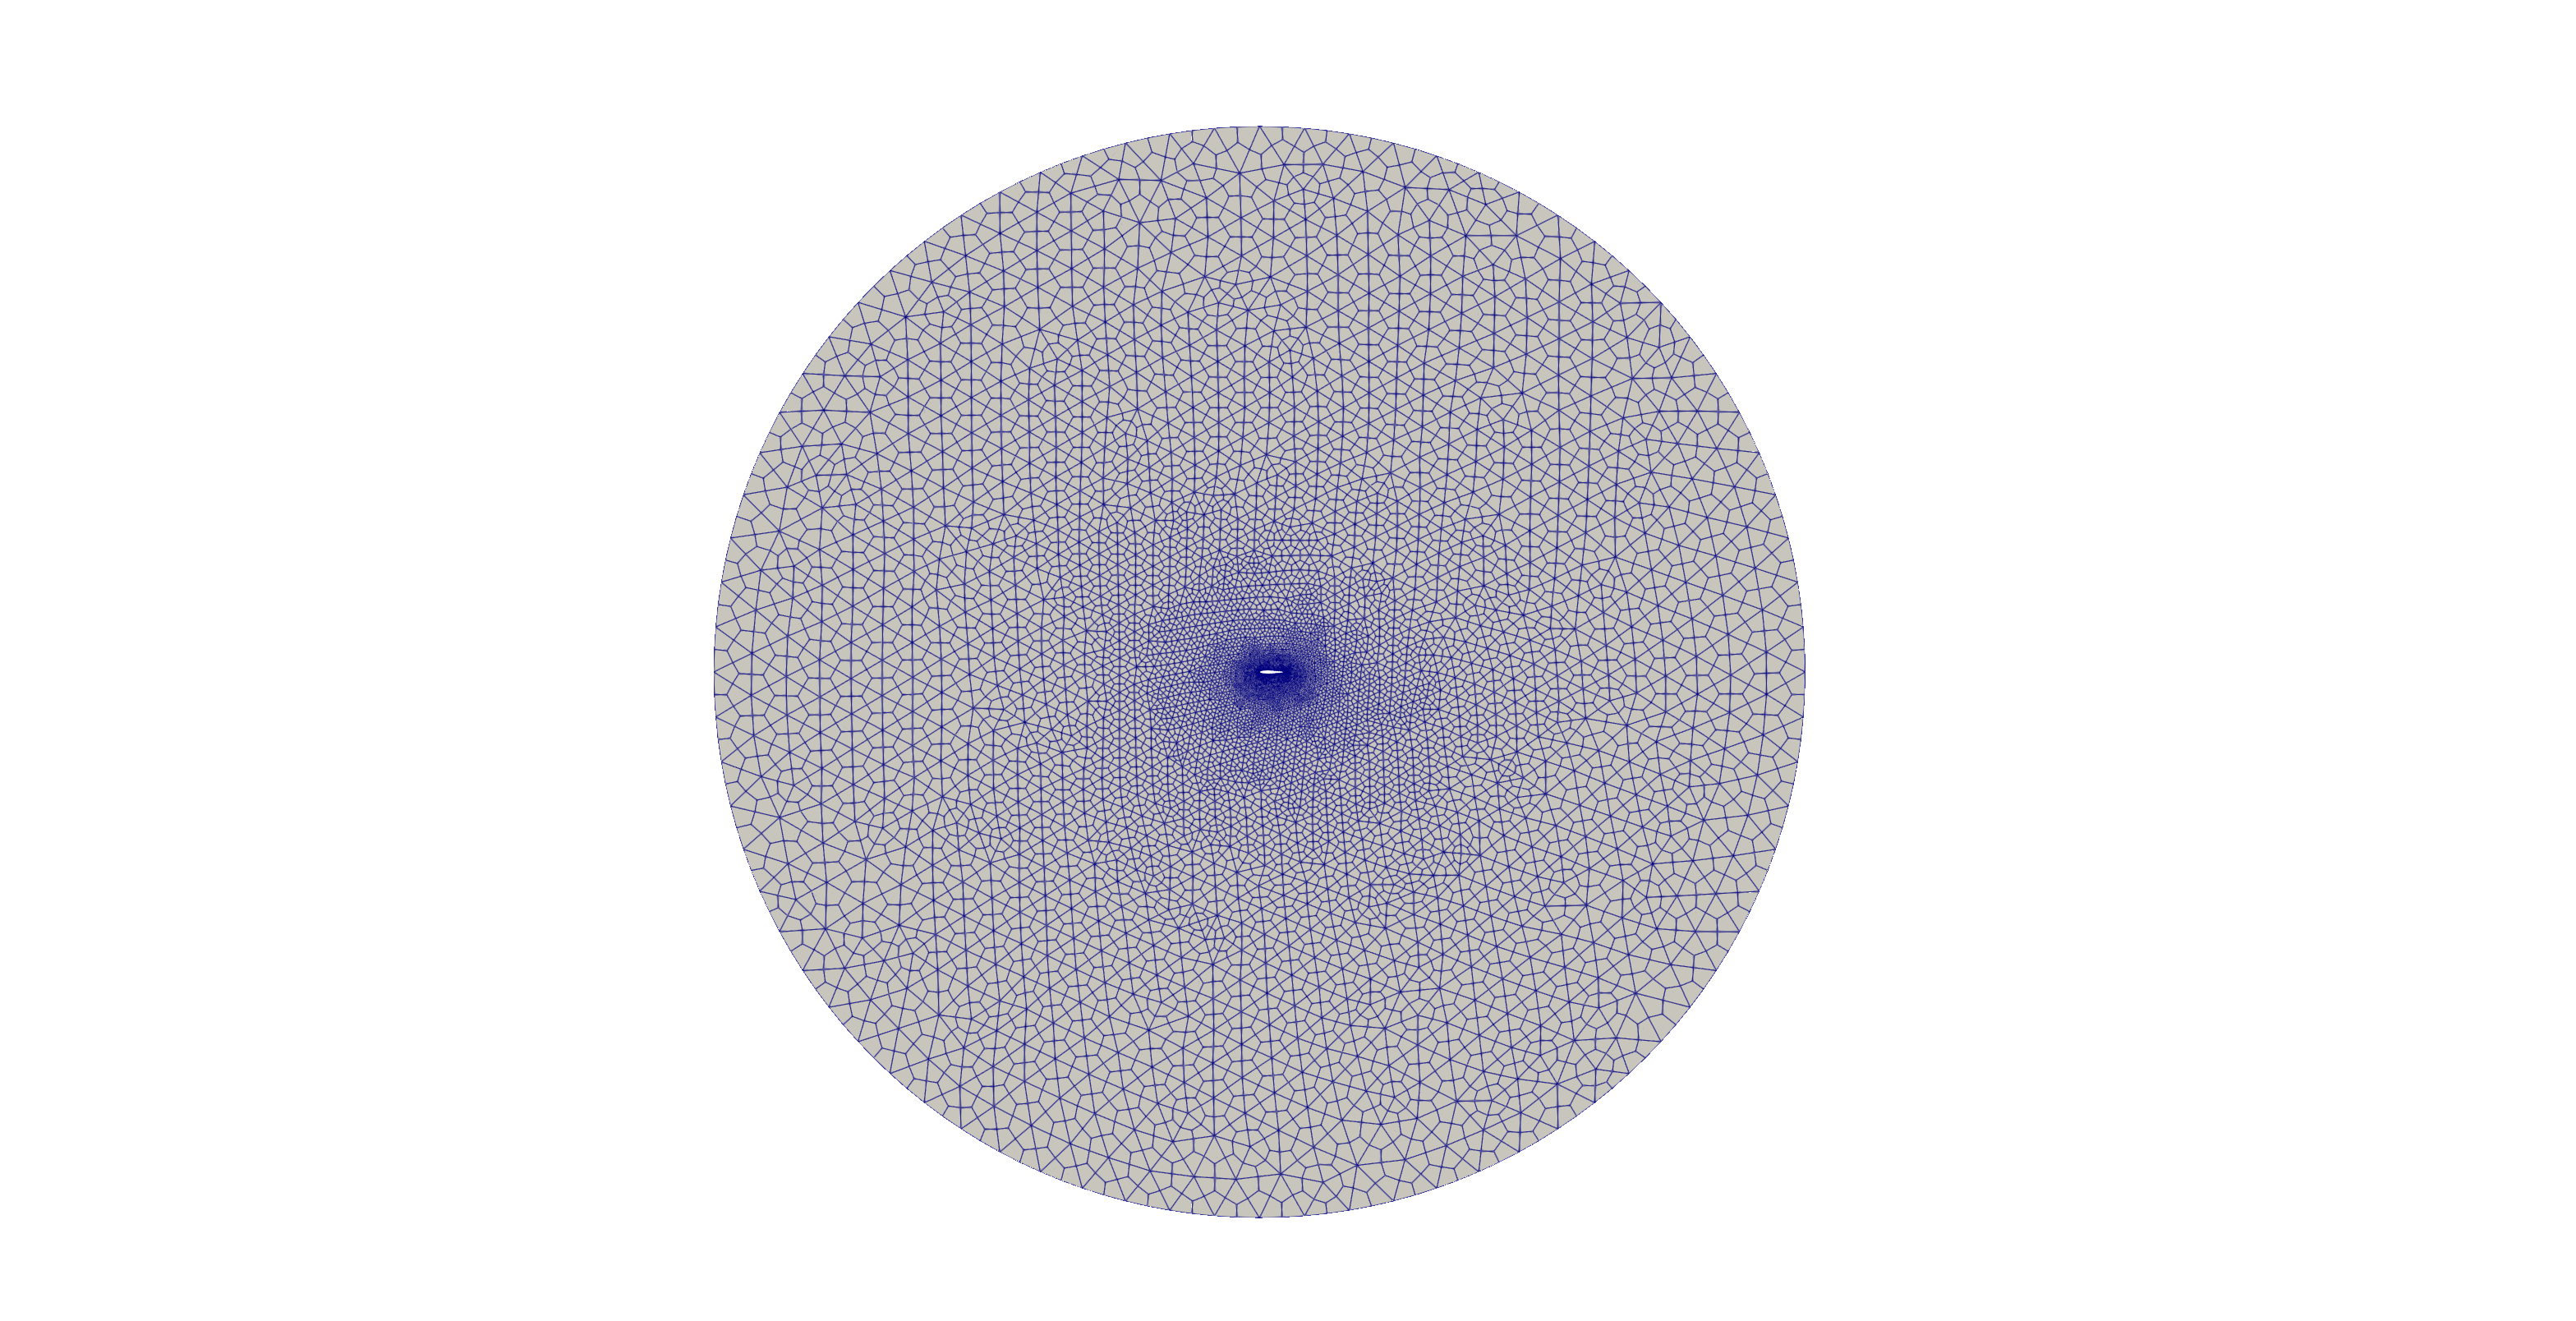
\includegraphics[width=0.45\textwidth]{Chapter_results/media/airfoil_mesh}\label{fig:complex_mesh_close}}
	\hfill
	\subfloat[Airfoil]
	{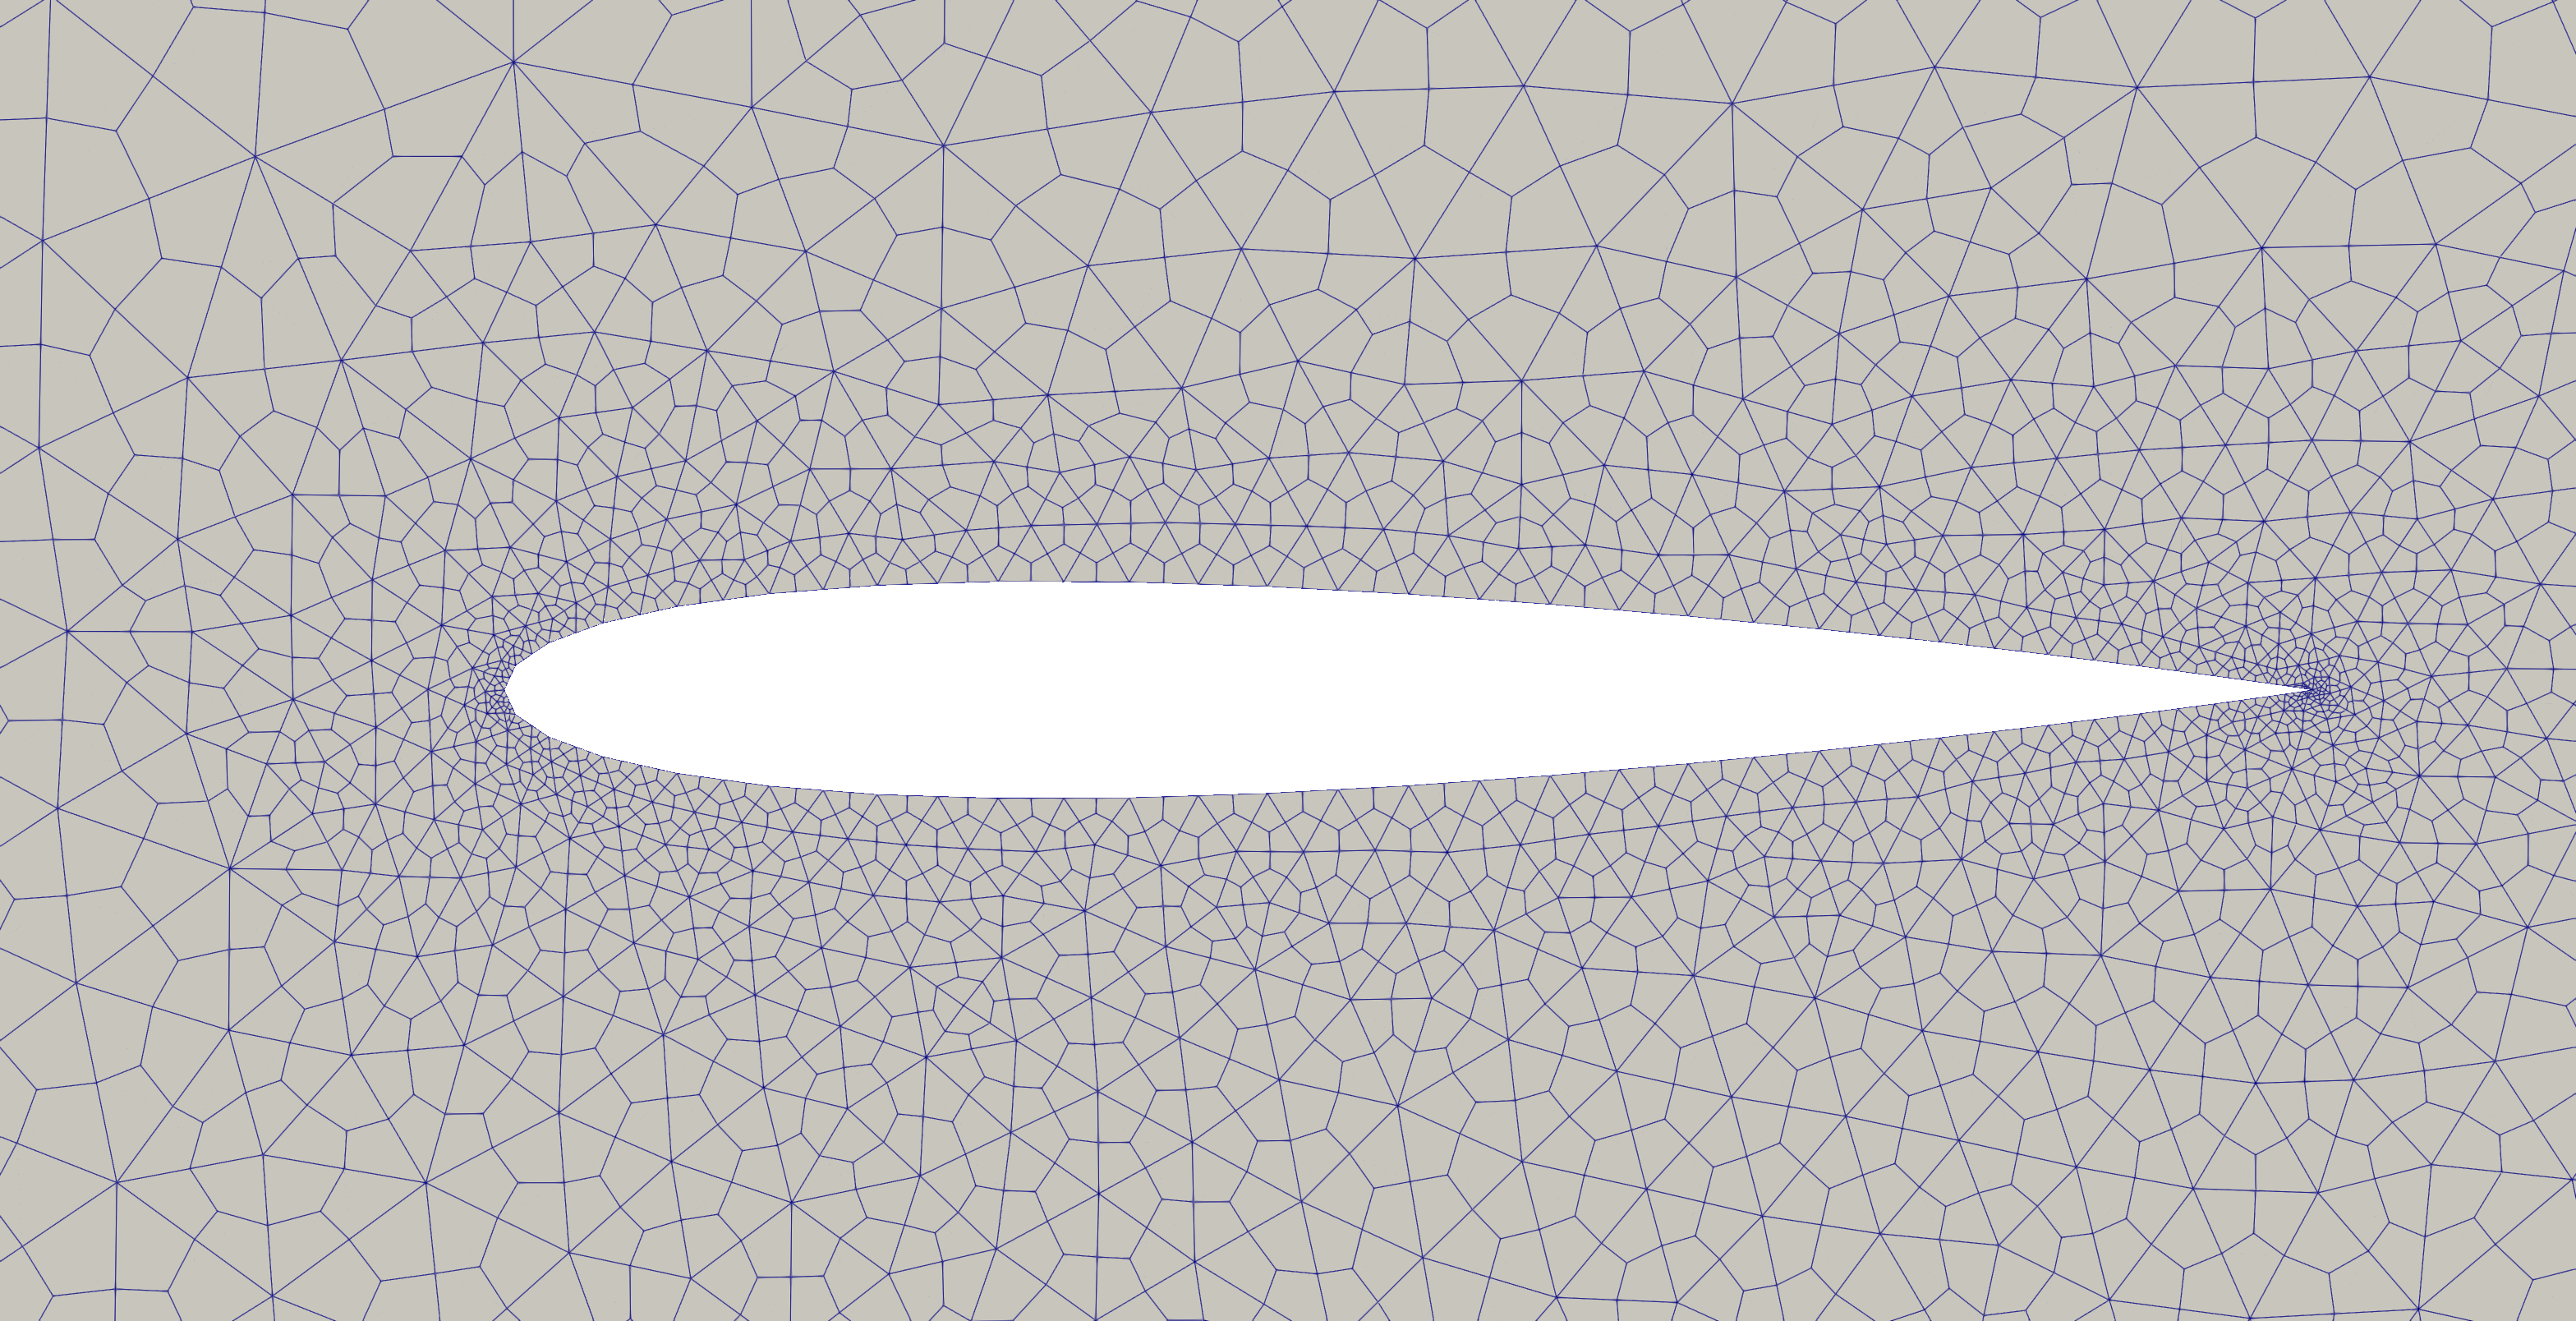
\includegraphics[width=0.45\textwidth]{Chapter_results/media/airfoil_mesh_close}\label{fig:complex_mesh_far}}
	\caption{Complex mesh: An airfoil in an unstructured circular domain. (a) Complete domain (b) Up close}\label{fig:complex_mesh}
\end{figure}

\begin{figure}[H]
	\centering
	\subfloat[Pressure]
	{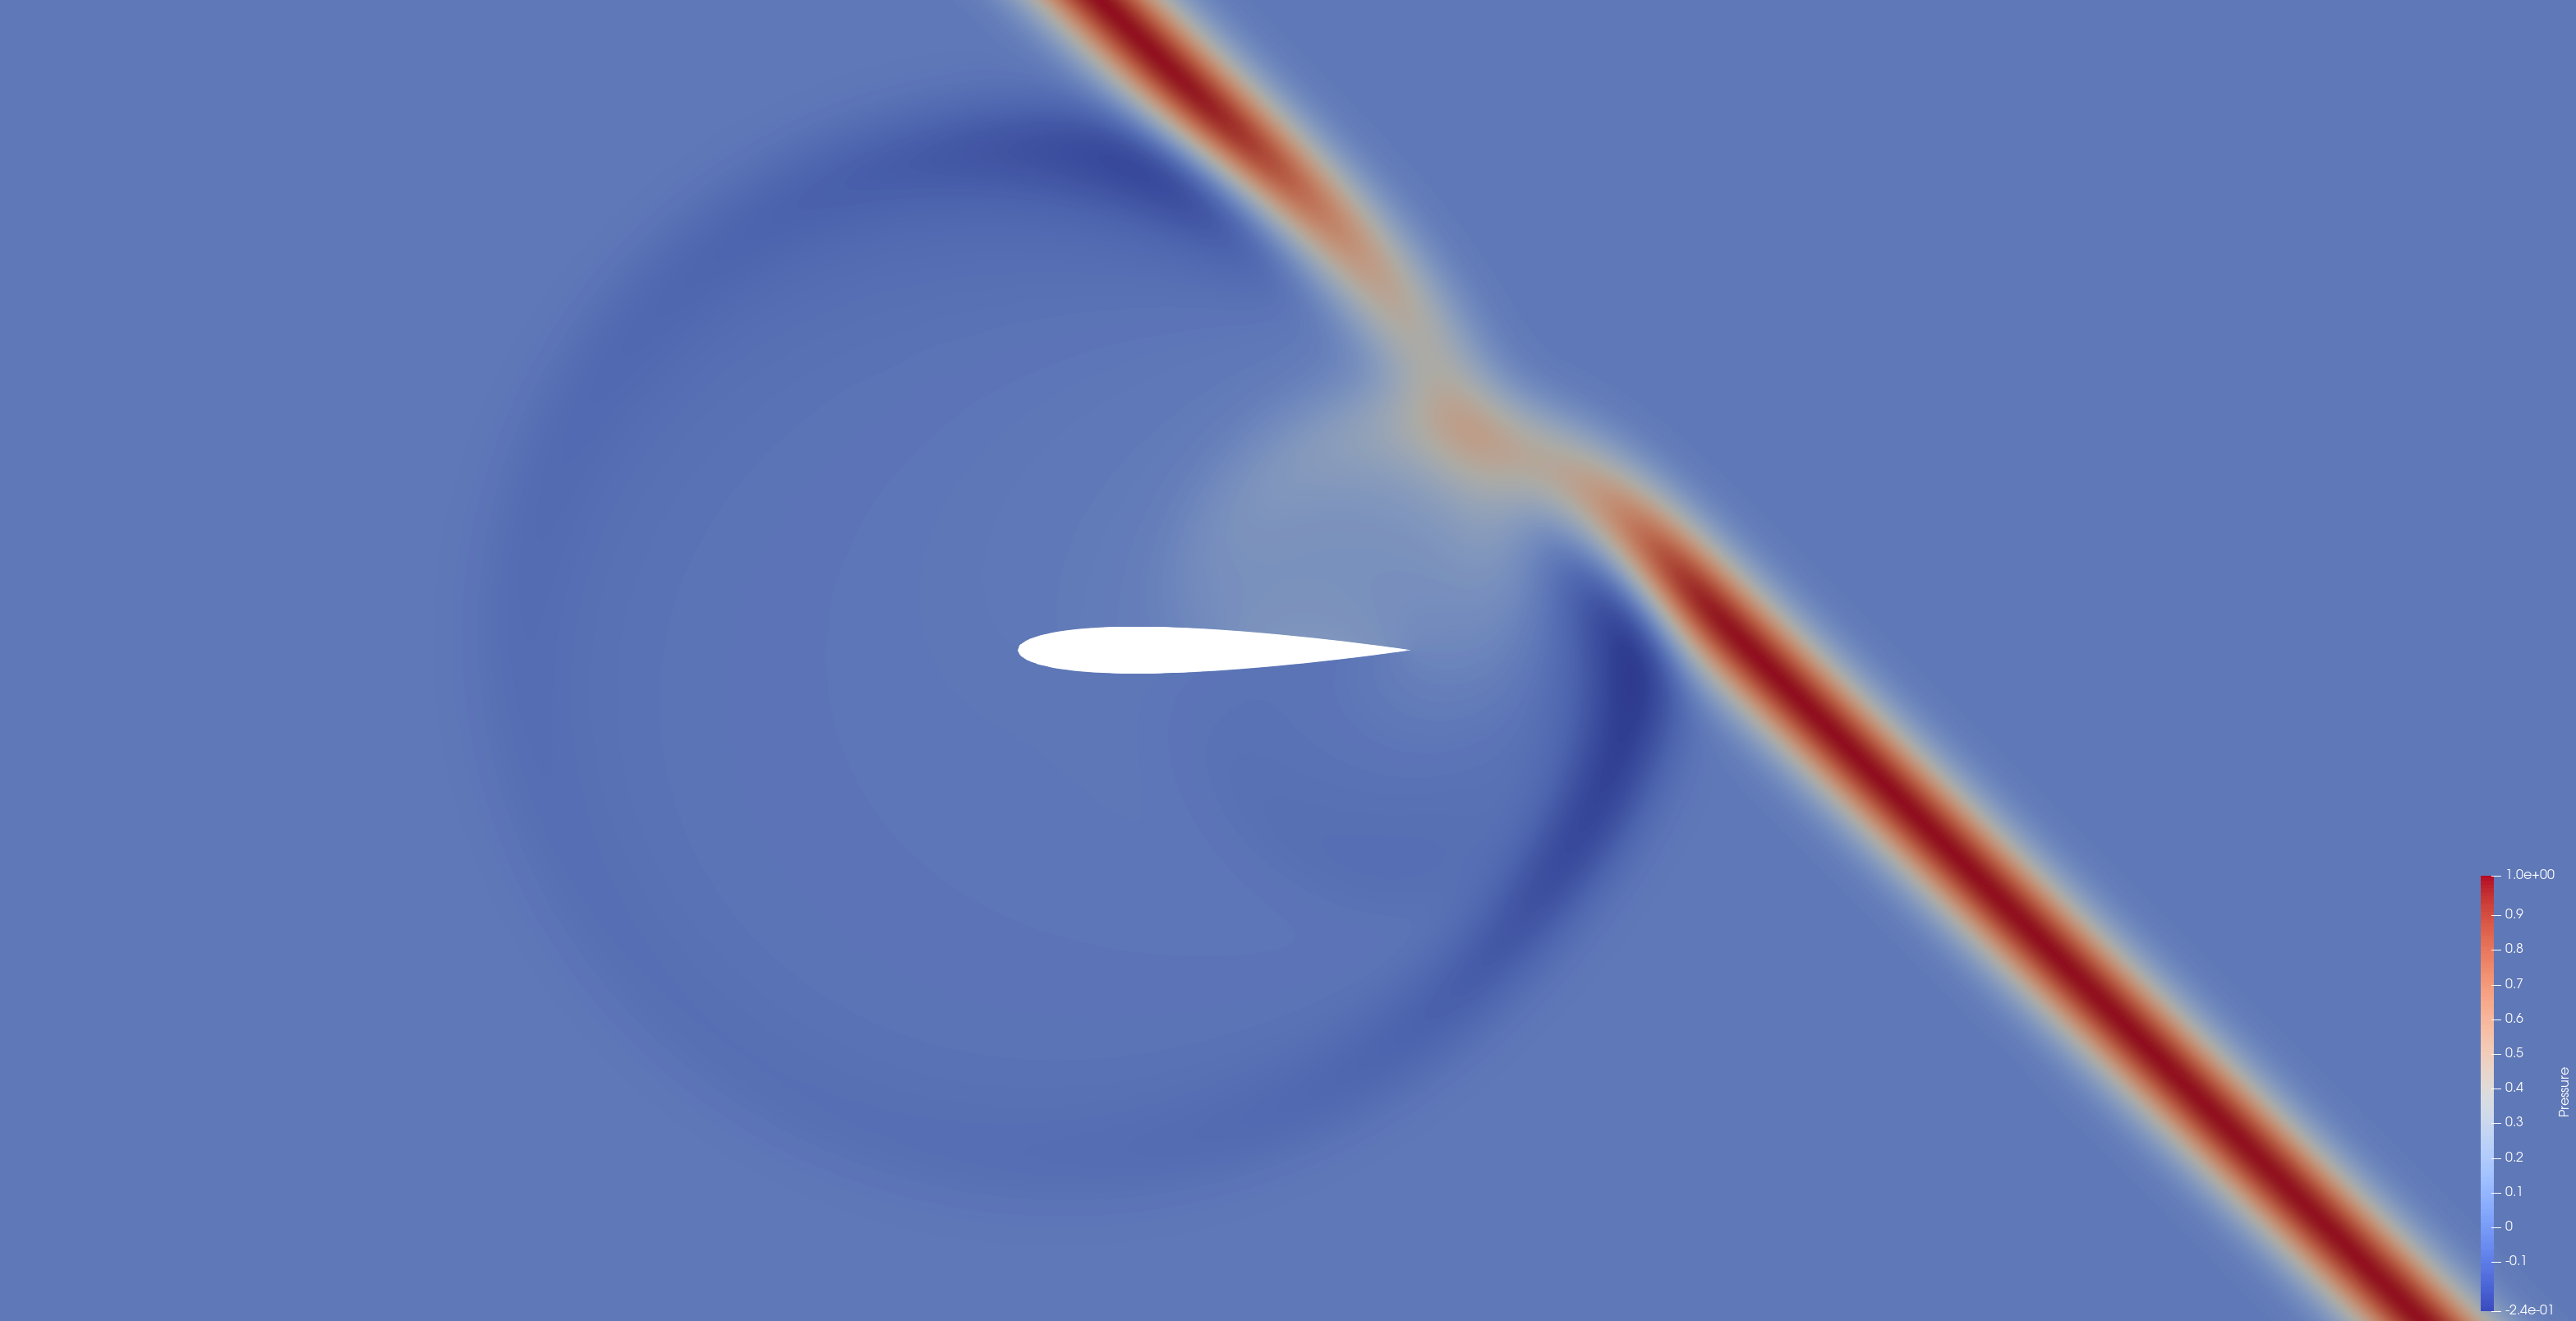
\includegraphics[width=0.45\textwidth]{Chapter_results/media/airfoil_pressure_close_t1_6}\label{fig:complex_mesh_solution_close}}
	\hfill
	\subfloat[Pressure \(\sigma \)]
	{
\includegraphics[width=0.45\textwidth]{Chapter_results/media/Airfoil 4}\label{fig:complex_mesh_solution_far}}
	\caption{Complex mesh: A wave going over an airfoil. (a) Pressure (b) Pressure \(\sigma \), denoting if h-refinement or p-refinement would be chosen}\label{fig:complex_mesh_solution}
\end{figure}
